\section{Postgres: Deleting database and restoring from PITR}
\label{app_pg_s2e1}



\begin{figure}[H]
    \centering
    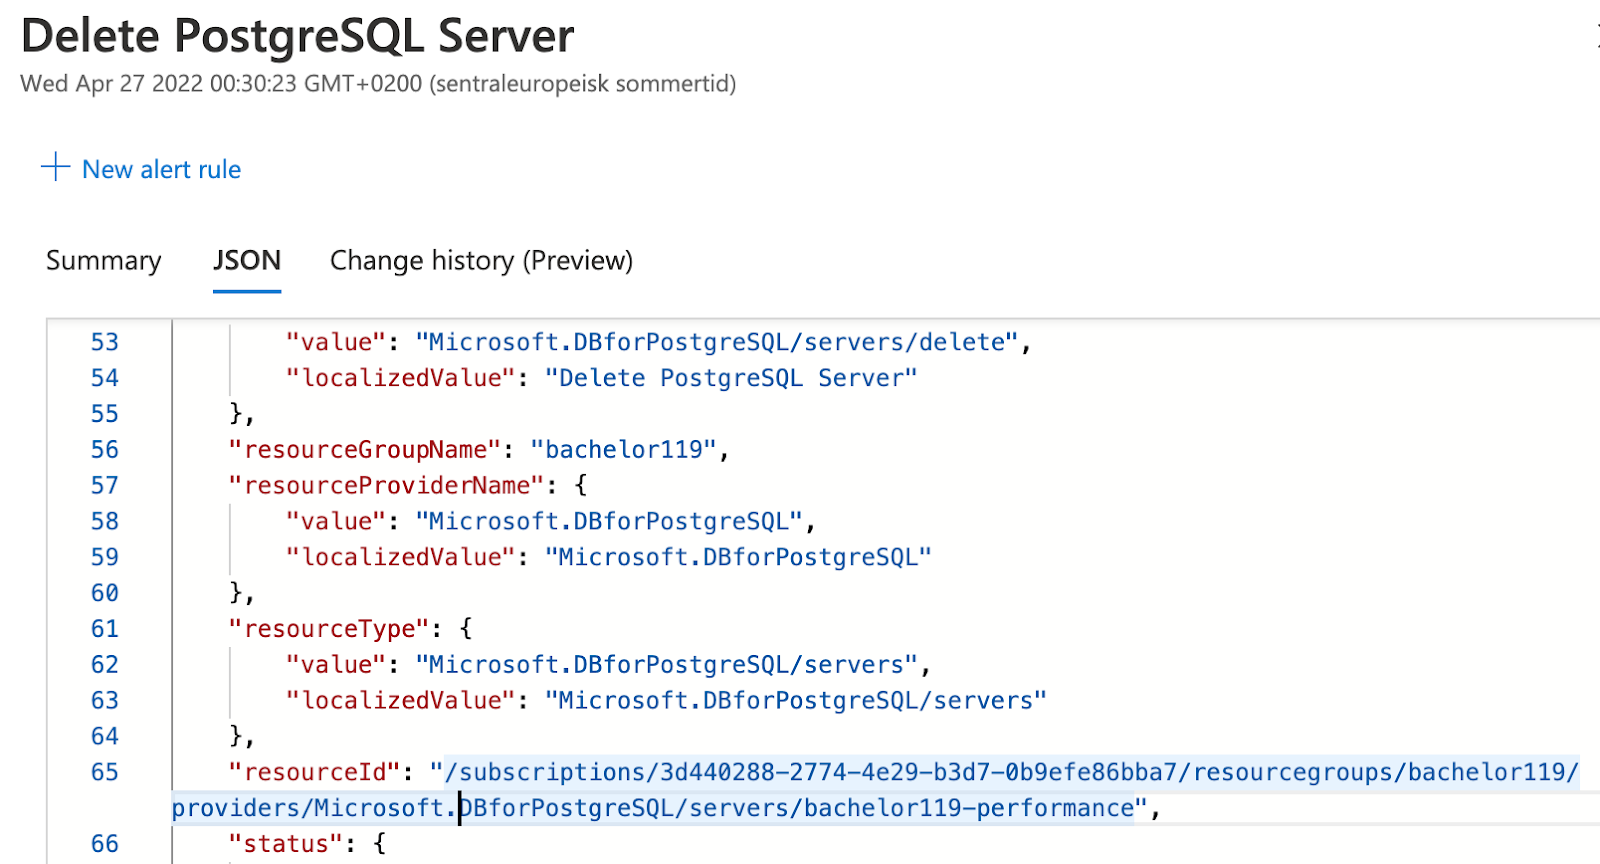
\includegraphics[width=\textwidth]{figures/postgres/delete_server.png}
    \caption{JSON output of the delete operation}
    \label{fig:my_label}
\end{figure}

However, this is a form of soft delete since the Azure backup ensures that it is possible to redeploy the server after deletion within the retention period of said server.
In addition, when creating the server the property of "createMode" can be set to "PointInTimeRestore". This can be done through the REST API endpoint for creating servers, where the resource ID of the deleted server has to be included in the request body. 
The resource ID of the deleted server can be found in the JSON file of the delete operation that should be stored in the Azure portal activity log. Below we demonstrate the recovery of the server. 
This way we establish that a server that was encrypted and then deleted still has the ability to fully recover to an operational pre-encryption state.

\begin{figure}[H]
    \centering
    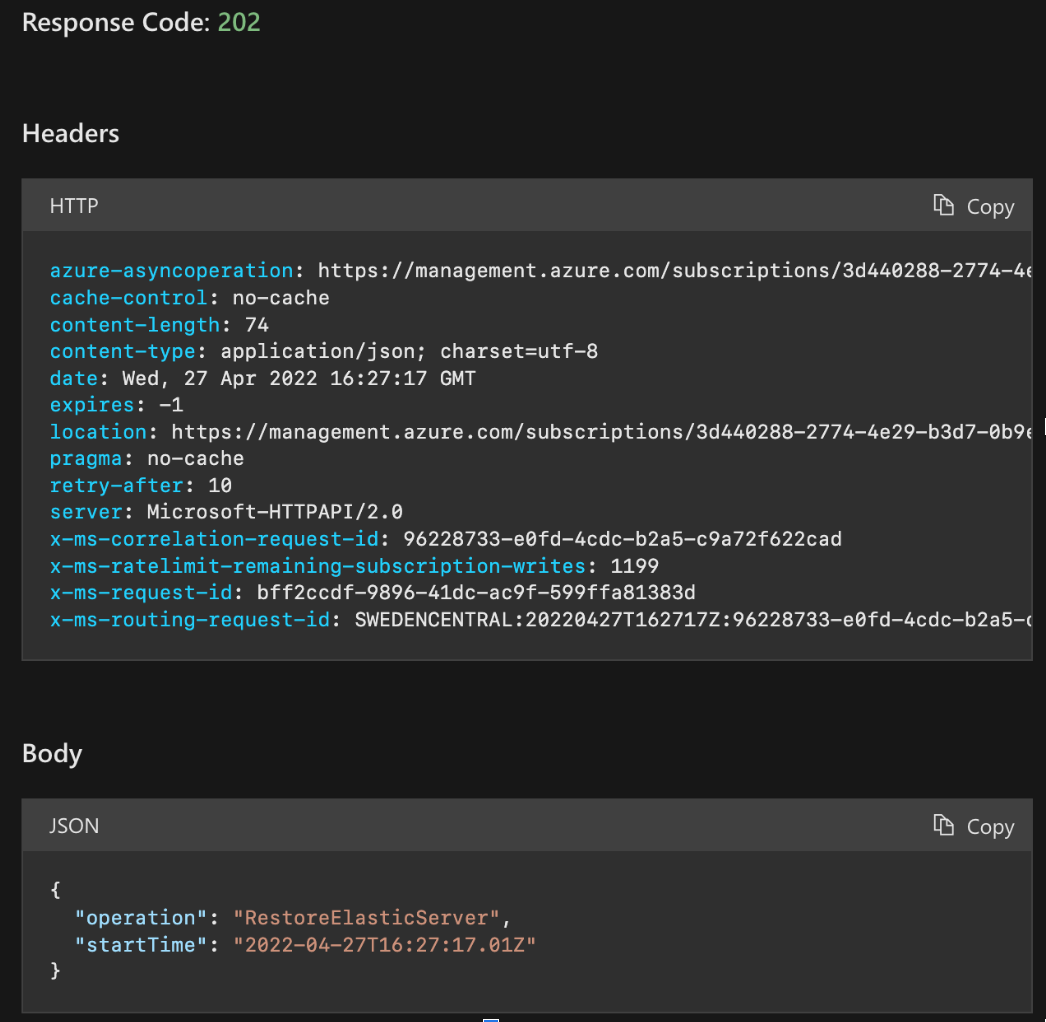
\includegraphics[width=\textwidth]{figures/postgres/recover_deleted_server.png}
    \caption{Summary of the API call}
    \label{fig:my_label}
\end{figure}

\begin{figure}[H]
    \centering
    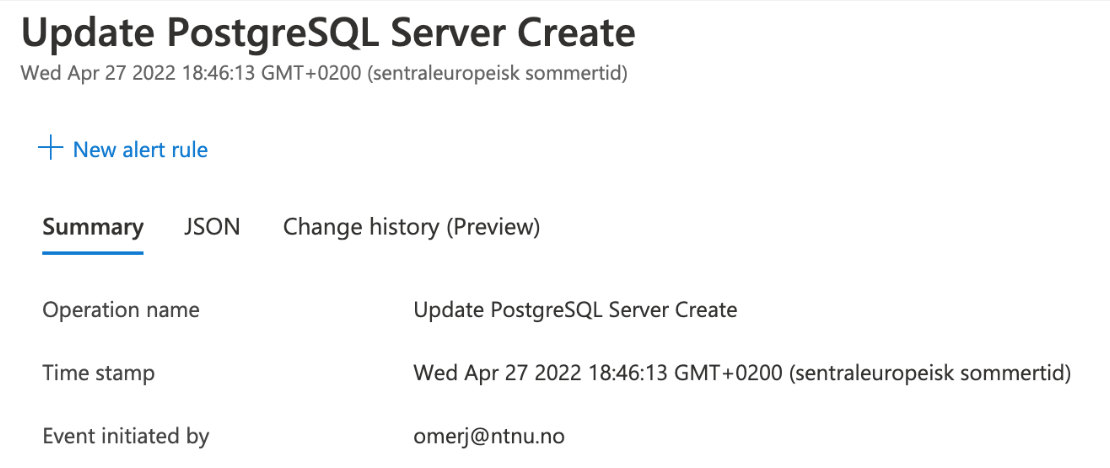
\includegraphics[width=\textwidth]{figures/postgres/scenario2_restored.png}
    \caption{Server created and database restored}
    \label{fig:my_label}
\end{figure}
